\documentclass[12pt,a4paper]{amsart}
\usepackage[slovene]{babel}
%\usepackage[cp1250]{inputenc}
\usepackage[T1]{fontenc}
\usepackage[utf8]{inputenc}
\usepackage{amsmath,amssymb,amsfonts}
\usepackage{url}
\usepackage[normalem]{ulem}
\usepackage[dvipsnames,usenames]{color}
\usepackage{graphicx}

% Oblika strani
\textwidth 15cm
\textheight 24cm
\oddsidemargin.5cm
\evensidemargin.5cm
\topmargin-5mm
\addtolength{\footskip}{10pt}
\pagestyle{plain}
\overfullrule=15pt % oznaci predlogo vrstico

% Ukazi za matematična okolja
\theoremstyle{definition} % tekst napisan pokončno
\newtheorem{definicija}{Definicija}[section]
\newtheorem{primer}[definicija]{Primer}
\newtheorem{opomba}[definicija]{Opomba}

\renewcommand\endprimer{\hfill$\diamondsuit$}


\theoremstyle{plain} % tekst napisan poševno
\newtheorem{lema}[definicija]{Lema}
\newtheorem{izrek}[definicija]{Izrek}
\newtheorem{trditev}[definicija]{Trditev}
\newtheorem{posledica}[definicija]{Posledica}

\begin{document}

%%%%%%%%%%%%%%%%%%%%%%%%%%%%%%%%%%%%%%%%%%%%%%%%%%%%%%%%%%%%%%%%%%%%%%%%%%%%%%%%%%%%%%%%%%%%%%%%%%%%%%%%%%%%%%%%%%%%%%%%%%%%%%%%%%%%%%%%%%%%%%
\title{Statistika v kazenskem pravu}
\author{Neža Kržan}
\maketitle

%%%%%%%%%%%%%%%%%%%%%%%%%%%%%%%%%%%%%%%%%%%%%%%%%%%%%%%%%%%%%%%%%%%%%%%%%%%%%%%%%%%%%%%%%%%%%%%%%%%%%%%%%%%%%%%%%%%%%%%%%%%%%%%%%%%%%%%%%%%%%%
%%%%%%%%%%%%%%%%%%%%%%%%%%%%%%%%%%%%%%%%%%%%%%%%%%%%%%%%%%%%%%%%%%%%%%%%%%%%%%%%%%%%%%%%%%%%%%%%%%%%%%%%%%%%%%%%%%%%%%%%%%%%%%%%%%%%%%%%%%%%%%
\section{Statistika v kazenskem pravu}
Raziskave na področju kazenskega pravosodja in kriminologije so različne po naravi in namenu. Velik del raziskav vključuje preverjanje teorije in hipotez.\\\\
Raziskovalci si prizadevajo preučiti razmerja med dvema ali več spremenljivkami. Opazovani ali empirični pojavi sprožajo vprašanja.\\\\
Odvisne spremenljivke so empirični dogodki, ki jih želi raziskovalec pojasniti. Neodvisne spremenljivke so dejavniki, za katere raziskovalec meni, da bi lahko vplivali na odvisne 
spremenljivke. Glede na naravo raziskovalne študije določimo neodvisne in odvisne spremenljivke.\\\\
Pomembno je razumeti, da neodvisno in odvisno nista sinonima za vzrok in posledico. Študije morajo izpolnjevati tri merila. Prvo je časovno zaporedje, kar pomeni, 
da se mora neodvisna spremenljivka pojaviti pred odvisno spremenljivko. 
Druga zahteva glede vzročnosti je, da obstaja empirična povezava med neodvisno spremenljivko in odvisno spremenljivko. Zadnja zahteva je, da je razmerje 
med neodvisno spremenljivko in odvisno spremenljivko nepristransko.\\\\
Statistični znanstveniki se že na začetku sodnega procesa soočajo s prvimi težavami - določitvijo odvisnih in neodvisnih spremenljivk za modeliranje. V 
proces določanja spremenljivk pa pogosto posežejo odvetniki, ki se sklicujejo na pravne zakone in načela. To lahko postane sporno, saj lahko takšni 
posegi ovirajo statistične znanstvenike pri izračunu verjetnostnega vpliva spremenljivk. Odvetniki imajo pomembno vlogo pri zagovarjanju strank v 
sodnih postopkih, vendar je njihovo znanje o statistiki in verjetnostnih izračunih omejeno. Po mojem mnenju zato odvetniki lahko napačno opredelijo 
odvisne in neodvisne spremenljivke ter s tem vplivajo na kakovost modeliranja. To pa lahko privede do napačnih zaključkov in napravilnih odločitev v 
sodnih postopkih. Ker so pravni zakoni pomembni, menim, da je sodelovanje med statistični znanstveniki in odvetniki potrebno. S tem se lahko zagotovi pravilno 
opredelitev spremenljivk in pravilne verjetnostne izračune, ki bodo prispevali k pravičnim odločitvam v sodnih postopkih.

%%%%%%%%%%%%%%%%%%%%%%%%%%%%%%%%%%%%%%%%%%%%%%%%%%%%%%%%%%%%%%%%%%%%%%%%%%%%%%%%%%%%%%%%%%%%%%%%%%%%%%%%%%%%%%%%%%%%%%%%%%%%%%%%%%%%%%%%%%%%%%
%%%%%%%%%%%%%%%%%%%%%%%%%%%%%%%%%%%%%%%%%%%%%%%%%%%%%%%%%%%%%%%%%%%%%%%%%%%%%%%%%%%%%%%%%%%%%%%%%%%%%%%%%%%%%%%%%%%%%%%%%%%%%%%%%%%%%%%%%%%%%%
\section{Uporaba statistike pri pravnem postopku}
Pred pričanjem na sodišču moramo vedeti, na kaj točno se podatki nanašajo, kako so bili zbrani in kakšen del manjka ali je neuporaben, da se lahko odločimo 
za ustrezen postopek analize podatkov. Potrebujemo osnovne informacije odvetnika in drugih strokovnjakov, da oblikujemo ustrezne primerjalne skupine. Ta 
postopek vključuje določitev ustrezne populacije (populacij), ki jo (jih) je treba preučiti, parametrov, ki nas zanimajo, in statističnega postopka, ki ga je 
treba uporabiti. \\\\
Statistične informacije, ki jih dobi sodnik, so filtrirane prek odvetnikov. Odvenik avtorju statistične analize postavlja vprašanja z namenom razlage 
statistične analize poroti, sodniku in drugim v sodni dvorani. Vprašanja so s strani odvetnikov seveda premišljeno postavljena, zato se lahko zgodi, da do 
temeljite razlage analize ne pride, ker analitik ne dobi primernih vprašanj. Kasneje bom obrazložila zmote, ki nastanejo zaradi pomankanja znanja verjetnosti 
pri sodnikih, poroti in odvetnikih, mogoče pa nekatere izmed njih nastanejo tudi zaradi nepopolne razlage statistične analize. Do neke točke analitik sicer sam 
predstavi analizo, potem pa mora biti tudi on previden z razlago, zaradi porote, kajti poroti se predvidoma ne govori kako naj si razlaga dokaze, kar pa ponavadi preučujemo 
s statistično analizo. Mogoče bi moralo biti določeno kaj vse mora analitik predstaviti in razložiti, da bi se lahko izognili zmotam.\\
Potrebno je kombiniranje različnih postopkov za pridobivanje informacij iz podatkov in razlago rezultatov, kar sem zasledila, da strokovnjaki velikokrat 
izkoriščajo, se ne poglobijo dovolj in predstavljena analiza postane nepopolna.

%%%%%%%%%%%%%%%%%%%%%%%%%%%%%%%%%%%%%%%%%%%%%%%%%%%%%%%%%%%%%%%%%%%%%%%%%%%%%%%%%%%%%%%%%%%%%%%%%%%%%%%%%%%%%%%%%%%%%%%%%%%%%%%%%%%%%%%%%%%%%%
%%%%%%%%%%%%%%%%%%%%%%%%%%%%%%%%%%%%%%%%%%%%%%%%%%%%%%%%%%%%%%%%%%%%%%%%%%%%%%%%%%%%%%%%%%%%%%%%%%%%%%%%%%%%%%%%%%%%%%%%%%%%%%%%%%%%%%%%%%%%%%
\section{Raziskovalni proces}
Raziskovalni proces v kazenskem pravosodju je običajno namenjen preučevanju problemov kriminala. Proces se izvaja po naslednjih točkah.\\
\textit{1. Identifikacija problema.\\} 
\textit{2. Zasnova raziskave.\\} 
\textit{3. Analiza podatkov.\\}

%%%%%%%%%%%%%%%%%%%%%%%%%%%%%%%%%%%%%%%%%%%%%%%%%%%%%%%%%%%%%%%%%%%%%%%%%%%%%%%%%%%%%%%%%%%%%%%%%%%%%%%%%%%%%%%%%%%%%%%%%%%%%%%%%%%%%%%%%%%%%%
%%%%%%%%%%%%%%%%%%%%%%%%%%%%%%%%%%%%%%%%%%%%%%%%%%%%%%%%%%%%%%%%%%%%%%%%%%%%%%%%%%%%%%%%%%%%%%%%%%%%%%%%%%%%%%%%%%%%%%%%%%%%%%%%%%%%%%%%%%%%%%
\section{Vrednotenje dokazov}
Postopek ugotavljanja dejstev zahteva oceno vseh dokazov, ki jih predložijo sodišču, da se določi, ali je obdolženec kriv 
ali ne. Uvede se pojem dokazni standard, ki je pravno vprašanje, tj. gre za abstraktno normo, ki je (podobno kot obstoj določenih predpostavk za 
določeno kaznivo dejanje) opredeljena s pravnim pravilom. Vrednotenje dokazov pa je t.i. dejansko vprašanje, gre za odločitev, kako se dokazi, v določenem 
primeru, nanašajo na normo. \\\\
Matematični pristopi za ocenjevanje dokazov določajo različne odstotke za dokazni standard, ki je manjši od popolne gotovosti, zato se 
predložene informacije (ali njihovo pomanjkanje) pretvorijo v številčno vrednost (običajno približno 90-95-odstotna stopnja verjetnosti), ki se nato 
primerja z zahtevanim dokaznim standardom.\\\\
Najpogostejši uporabljeni metodi za ocenjevanje dokazov sta metoda dokazne vrednosti in model verjetnosti hipoteze.
V kazenskem pravu pa lahko zelo hitro pride do posebnih, edinstvenih predpostavk oziroma hipotez, ki pa predstavljajo težave pri vrednotenju oziroma 
merjenju v statističnih modelih. 

%%%%%%%%%%%%%%%%%%%%%%%%%%%%%%%%%%%%%%%%%%%%%%%%%%%%%%%%%%%%%%%%%%%%%%%%%%%%%%%%%%%%%%%%%%%%%%%%%%%%%%%%%%%%%%%%%%%%%%%%%%%%%%%%%%%%%%%%%%%%%%
%%%%%%%%%%%%%%%%%%%%%%%%%%%%%%%%%%%%%%%%%%%%%%%%%%%%%%%%%%%%%%%%%%%%%%%%%%%%%%%%%%%%%%%%%%%%%%%%%%%%%%%%%%%%%%%%%%%%%%%%%%%%%%%%%%%%%%%%%%%%%%
\section{Koncept verjetnosti}
Pogosto se opravlja primerjava verjetnosti dokazov na podlagi dveh konkurenčnih predlogov, in sicer predloga tožilca in predloga obrambe.\\\\
$H_p \dots$ trditev, ki jo predlaga tožilstvo;\\
$H_d \dots$ trditev, ki jo predlaga obramba;\\\\
Pri presoji dokazov se najprej analizira njihova verjetnost. Dokazi se ne presojajo izolirano, ampak v kontekstu celotnega primera. V skladu s konceptom 
verjetnosti se pri presoji dokazov upošteva tudi verjetnost napake. Verjetnost napake se nanaša na verjetnost, da so dokazi napačni ali zavajajoči. V splošnem 
nas zanima vpliv dokazov na verjetnost krivde($H_p$) in nedolžnosti($H_d$) osumljenca. Gre za dopolnjujoča se dogodka in razmerje verjetnosti teh dveh dogodkov,
\begin{equation}
   \frac{P(H_p)}{P(H_d)}, \vspace{2mm}
\end{equation}
je verjetnost proti nedolžnosti ali verjetnost za krivdo. Ob upoštevanju dodatnih informacij $E$ oziroma dokazov, je razmerje
\begin{equation}
   \frac{P(H_p \lvert E)}{P(H_d \lvert E)} \vspace{2mm},
\end{equation}
verjetnost v prid krivdi ob upoštevanju informacij $E$.\\\\
Če imamo na voljo dokaz $E$, nas zanima pogojna verjetnost
\[
    P(kriv \lvert E), \vspace{2mm}
\]
pri čemer nam je lahko v pomoč Bayesovo pravilo. To v teoriji drži, čeprav je v praksi izračun verjetnostne krivde lahko preveč zapleten. Ampak 
z Bayesovim pravilom lahko ocenimo verjetnosti vmesnih trditev oziroma dokazov, ki so ključnega pomena za ugotavljanje obtoženčeve krivde.

%%%%%%%%%%%%%%%%%%%%%%%%%%%%%%%%%%%%%%%%%%%%%%%%%%%%%%%%%%%%%%%%%%%%%%%%%%%%%%%%%%%%%%%%%%%%%%%%%%%%%%%%%%%%%%%%%%%%%%%%%%%%%%%%%%%%%%%%%%%%%%
%%%%%%%%%%%%%%%%%%%%%%%%%%%%%%%%%%%%%%%%%%%%%%%%%%%%%%%%%%%%%%%%%%%%%%%%%%%%%%%%%%%%%%%%%%%%%%%%%%%%%%%%%%%%%%%%%%%%%%%%%%%%%%%%%%%%%%%%%%%%%%
\section{Bayesova statistika}

%%%%%%%%%%%%%%%%%%%%%%%%%%%%%%%%%%%%%%%%%%%%%%%%%%%%%%%%%%%%%%%%%%%%%%%%%%%%%%%%%%%%%%%%%%%%%%%%%%%%%%%%%%%%%%%%%%%%%%%%%%%%%%%%%%%%%%%%%%%%%%
\subsection{Bayesova teorija v kazenskem pravu}
Bayesova teorija razlaga verjetnost kot merilo verjetnosti ali zaupanja, ki ga lahko ima posameznik glede nastanka določenega dogodka.
O nekem dogodku lahko že imamo predhodno prepričanje oziroma apriorno prepričanje, ki pa se lahko spremeni, ko se pojavijo novi dokazi. Daje nam
matematične modele za vključevanje naših apriornih prepričanj in dokazov za ustvarjanje novih prepričanj oziroma za pridobitev a posteriori
prepričanja, ki se lahko uporabi za kasnejše odločitve.\\\\
Sodniki ali porotniki, ki ugotavljajo sklep sodbe, imajo na voljo vrsto dokazov. Njihova naloga je ocena, kako te informacije vplivajo na tožilčevo
domnevo o obdolžencu oziroma storilcu kaznivega dejanja. Pri Bayesovi teoriji moramo upoštevati vsak dokaz posebej, kar je še posebej pomembno pri
začetku sodbe. Pomembno je tudi, da razlikujemo med dokazi pri Bayesovi teoriji in dokazi na sodišču. V Bayesovi teoriji je vsaka informacija
dokaz, če je pomembna za verjetnost hipoteze. V kazenskem postopku pa je dokaz informacija, ki je bila predložena sodišču za podporo določeni
izjavi na sodišču in je sprejeta kot pravno dopustna, kar pomeni, da je ta informacija znana sodniku, ki presoja tožilčevo domnevo o obdolžencu in je
pomembna za verjetnost hipoteze.

%%%%%%%%%%%%%%%%%%%%%%%%%%%%%%%%%%%%%%%%%%%%%%%%%%%%%%%%%%%%%%%%%%%%%%%%%%%%%%%%%%%%%%%%%%%%%%%%%%%%%%%%%%%%%%%%%%%%%%%%%%%%%%%%%%%%%%%%%%%%%%
\subsection{Predhodna verjetnost in določitev posteriorne verjetnosti}
Predhodna verjetnost, ki je uporabljena v vsaki posodobitvi verjetnosti s pomočjo Bayesove teorije, je začetna verjetnost hipoteze oziroma tožilčeve domneve 
o obdolžencu oziroma storilcu kaznivega dejanja. Razjasniti je potrebno tudi to, da ko odvetniki govorijo o predhodni verjetnosti, pogosto mislijo na verjetnost 
začetne hipoteze oziroma tožilčeve domneve o obdolžencu, preden so bili predloženi dokazi, kar je v skladu z opredelitvijo predhodne verjetnosti v Bayesovi 
teoriji. Po končni posodobitvi dobimo verjetnost hipoteze glede na vse dokaze, predložene na sojenju.\\\\
Recimo, da je statistični znanstvenik naprošen, da opravi analizo profila DNK krvi, najdene na kraju kaznivega dejanja, in rezultat primerja s profilom DNK
obdolženca. O krivdi ali nedolžnosti obtoženca bo odločala porota. Odločitev porotnikov bo delno odvisna od njihove ocene dveh interesnih
hipotez\\
$H_1 \dots$ vir krvi je obtoženec,\\
$H_2 \dots$ vir krvi je druga oseba.\\
Porotniki bodo morda želeli, da jim dokončno povemo, katera hipoteza je resnična, ali da jim navedemo verjetnosti vira. Za oceno verjetnosti 
vira mora statistični znanstvenik upoštevati tudi druge dokaze v kazenskem primeru.\\\\
Recimo, da je analitik ugotovil, da imata obtoženec in kri s kraja zločina skupen niz t.i. genetskih označevalcev, ki jih najdemo pri eni osebi
na 1 milijon prebivalcev v zadevni populaciji. Ne da bi upošteval druge dokaze, lahko analitik poda izjavo o pogojni verjetnosti
ugotovitve teh rezultatov pri dveh hipotezah o medsebojni povezanosti. analitik lahko na primer izjavi, da so skupni genetski označevalci
skoraj zagotovo najdeni v primeru $H_1$ (vir je bil obtoženec), vendar imajo le 1 možnost na milijon, da bodo najdeni v primeru $H_2$ (vir je bil
nekdo drug). Na podlagi te ocene lahko analitik poroti predloži razmerje verjetnosti - na primer, da so rezultati profila DNK 1 milijonkrat
bolj verjetni, če je bil vir krvi obtoženec in ne neka druga oseba. Vendar razmerje verjetnosti ni isto kot verjetnost vira. \\
Edini skladen način, kako na podlagi forenzičnih dokazov sklepati o verjetnosti virov, je uporaba Bayesovega pravila, ki zahteva, da začnemo s
pripisom predhodnih verjetnosti za hipoteze, ki nas zanimajo.\\\\
Določitev predhodnih oziroma apriornih verjetnosti je resen problem pri Bayesovemu pristopu v kazenskih postopkih. Različne metode za določitev in izračun teh 
verjetnosti lahko dajejo rezultate, ki se med seboj precej razlikujejo, kar pa je problematično, ker celotna Bayesova teorija temelji ravno na teh začetnih 
izračunih. Bistveno vprašanje, ki se postavlja, je, ali naj analitiki sploh poskušajo določiti predhodne verjetnosti in če ja, kako naj jih določijo. Nekateri 
strokovnjaki predlagajo, da bi analitiki morali predpostaviti enake predhodne verjetnosti za vse hipoteze v primeru, kar se imenuje nevtralno 
stanje. Torej analitiki predpostavljajo, da sta predhodni verjetnosti $H_1$ in $H_2$ enaki, nato pa 
ju v skladu z Bayesovim pravilom pomnožijo z razmerjem verjetnosti, da določijo posteriorno verjetnost. To bi se lahko izkazalo za praktičen pristop, 
saj se lahko analitik s tem izogne vplivu lastnih in odvetnikovih predsodkov ter mnenj, ki bi lahko vplivali na predpostavke o verjetnostih. Na ta način se 
lahko zagotovi objektivnost analize, saj ne poskušamo prikazati ene hipoteze bolj verjetne od druge. Kljub temu pa mislim, da moramo biti do tega 
pristopa nekoliko kritični, saj je predpostavljanje enake verjetnosti za vse možnosti problematično - v realnosti se različne hipoteze razlikujejo po svoji 
verjetnosti.\\
Mnenje in poročila statističnih znanstvenikov oziroma analitikov naj bi bila ključni vir informacij, ki lahko prispevajo k objektivnemu in strokovnemu 
vrednotenju dokazov in verjetnosti v sodnih postopkih. Zato sem mnenja, da je potrebno zagotoviti neodvisnost in strokovnost analitikov ter jih 
zaščititi pred morebitnim poseganjem odvetnikov ali drugih udeležencev sodnega postopka v njihov proces dela, tako kot morajo to zagotoviti oni. Analitik naj uporabi svoje strokovno znanje za izračun apriorne verjetnosti na podlagi razpoložljivih podatkov in brez nepotrebnega 
vplivanja odvetnikov ali drugih udeležencev postopka. Poleg tega sem ugotovila, da za statistiko v kazenskem pravu obstajajo pravila in smernice kako upoštevati zakonodajo, pravila 
in postopke sodbe, ki jih po mojem mnenju analitiki dosledno upoštevajo. Glavni očitek temu pristopu v okviru kazenskega postopka bi lahko bil, da lahko analitiki presežejo svoje znanstveno 
znanje in si prisvojijo vlogo tistega, ki ugotavlja dejstva, ampak vseeno predlagam, da odveniki nimajo nobene vloge pri ocenjevanju predhodnih verjetnosti.\\\\
Ko na nek način le določimo predhodne oziroma apriorne verjetnosti tožilčeve hipoteze in dokazov torej sledi posodabljanje le teh. Tekom sodbe se v realnosti vedno 
pojavljajo nove domneve o obtožencu in skoraj vedno najdejo nove dokaze s kraja zločina. Smiselno je, da vse to v postopku izračuniv tudi upoštevamo. Zasledila sem, da 
se tekom sodbe marsikateri dokaz najprej prizna in je znan sodniku, ki presoja tožilčevo domnevo o obdolžencu, torej ga analitik upošteva v svojih izračunih za posodobitve 
predhodnih verjetnosti hipotez. Potem pa dokaz iz sodbe umaknejo, ampak presnetilo me je, da dokaz največkrat ni umaknjen iz verjetnostnih računov. Mnenja sem, da bi 
morali anlitiki, ko se določen dokaz iz sodbe, zaradi tehtnega razloga, umakne, posodobiti vse račune za nazaj in nato nadaljevati posodabljanje verjetnosti. 

%%%%%%%%%%%%%%%%%%%%%%%%%%%%%%%%%%%%%%%%%%%%%%%%%%%%%%%%%%%%%%%%%%%%%%%%%%%%%%%%%%%%%%%%%%%%%%%%%%%%%%%%%%%%%%%%%%%%%%%%%%%%%%%%%%%%%%%%%%%%%%
%%%%%%%%%%%%%%%%%%%%%%%%%%%%%%%%%%%%%%%%%%%%%%%%%%%%%%%%%%%%%%%%%%%%%%%%%%%%%%%%%%%%%%%%%%%%%%%%%%%%%%%%%%%%%%%%%%%%%%%%%%%%%%%%%%%%%%%%%%%%%%
\section{Drugi pristopi}

%%%%%%%%%%%%%%%%%%%%%%%%%%%%%%%%%%%%%%%%%%%%%%%%%%%%%%%%%%%%%%%%%%%%%%%%%%%%%%%%%%%%%%%%%%%%%%%%%%%%%%%%%%%%%%%%%%%%%%%%%%%%%%%%%%%%%%%%%%%%
\subsection{Frekvence}
Predlagano je bilo s strani mnogih avtorjev, da je bolj naraven način za obravnavo verjetnosti uporaba naravnih frekvenc.\\
V forenzičnem kontekstu se frekvence običajno nanašajo na pojavljanje dokazov za posamezen primer, medtem ko se frekvence za
pojavljanje vprašanj običajno opisujejo kot osnovne stopnje. Sklepanje o krivdi je lahko podprto s statistično analizo
ustreznih podatkov in verjetnostnim sklepanjem z uporabo absolutnih ali relativnih frekvenc, pri čemer je verjetnost, da bi določene
podatke (dokaze) pridobili zgolj po naključju, izjemno majhna. Relativne frekvence vedno navajajo ali predpostavljajo, da obstaja nek
referenčni vzorec, na podlagi katerega se lahko oceni pogostost zadevnega dogodka. Nadaljnja predpostavka je, da je ta primerjava poučna
in pomembna za obravnavano nalogo. V okviru kazenskega postopka bi na primer pričakovali, da bo relativna frekvenca lahko podprla
vmesno sklepanje o moči dokazov, ki se nanašajo na sporna dejstva, kar vodi do končnega sklepa, da je obtoženec nedolžen ali kriv. Relativne
frekvence so rutinsko vključene v znanstvene dokaze, ki se predložijo v kazenskih postopkih.\\\\
S primera, ki sem ga naredila z obema metodama (frekvence in Bayesovo parvilo), sem videla, da so razlike zelo majhne, nekje pa jih celo ni.  Obe metodi, 
se lahko uporabljajo za reševanje določenih problemov, vendar se razlikujeta v načinu delovanja. Tako pri metodi edinstvenosti ni mogoče enostavno 
upoštevati številnih zapletov, kot je vpliv stopnje laboratorijskih napak. Bayesovo pravilo pa namreč omogoča upoštevanje različnih dejavnikov in 
zapletov, ki vplivajo na verjetnost določenega dogodka, s tem pa omogoča tudi bolj natančne izračune in posledično bolj zanesljive rezultate. Kljub 
temu pa ima tudi Bayesovo pravilo svoje omejitve, saj je odvisno od predpostavk in podatkov, ki jih uporabimo za izračun verjetnosti. V vsakem primeru je 
izbira metode odvisna od specifičnih zahtev problema in od tega, katera metoda bo najbolj primerna za njegovo reševanje.\\\\
Bistvena teoretična pomanjkljivost frekvenčnih modelov je, 
da zahtevajo statistične dokaze, ki sodišču niso na voljo. Sodišča ne morejo številčno ovrednotiti nekega dejanskega dokaza, saj se ne zavedajo možnih 
anomalij pri uporabi drugih sredstev in storitev. Poleg tega frekvenčni modeli temeljijo na predpostavki, da visoka vrednost verjetnosti, ki opisuje razmerje 
med obstoječimi dokazi in primerom, pomeni, da je vrednost tega dokaza visoka. Vendar to ni nujno vedno res. Merjenje skladnosti med dejanskimi dokazi 
in tistim, kar se je resnično zgodilo, temelji na predpostavki, da obstajata reprezentativna populacija in skladen rezultat. V kazenskem primeru pa 
ti pogoji niso izpolnjeni, kar pomeni, da je uporaba frekvenčnih modelov lahko omejena.

%%%%%%%%%%%%%%%%%%%%%%%%%%%%%%%%%%%%%%%%%%%%%%%%%%%%%%%%%%%%%%%%%%%%%%%%%%%%%%%%%%%%%%%%%%%%%%%%%%%%%%%%%%%%%%%%%%%%%%%%%%%%%%%%%%%%%%%%%%%%%%
\subsection{Metoda verjetnosti naključnega ujemanja}
Metoda verjetnost naključnega ujemanja izraža možnost, da bi imel naključni posameznik, ki ni povezan z obdolžencem,
ustrezni DNK profil. Ta verjetnost je enaka pogostosti profila DNK. Težava tega pristopa je, da verjetnost naključnega ujemanja lahko predstavljena
oziroma razumevana narobe. \\
Pogosto se to verjetnost interpretira na slednji način:
\begin{enumerate}
   \item če je verjetnost naključnega ujemanja na primer 1 proti 100 milijonom, potem je verjetnost, da ima profil DNK drug posameznik in ne
   obdolženec 1 proti 100 milijonom;
   \item ker je to zelo majhna verjetnost, mora biti tudi verjetnost, da je sled DNK pustil nekdo drug na kraju zločina in ne obdolženec, zelo majhna;
   \item zato mora biti verjetnost, da je vir sledi DNK s kraja zločina obtoženec zelo velika, ampak znaša 1 proti 100 milijonov.
\end{enumerate}
Takšno sklepanje je napačno in je znano kot tožilčeva zmota. Sestavlja jo enačba
\begin{equation}\label{eq:tozilcevazmota}
   1 - f = P(S \lvert M). \vspace{2mm}
\end{equation}
Zmota se pojavi v koraku (2), ko je zamenjano $P(M \lvert \neg S)$ s $P(\neg S \lvert M)$ in predpostavljeno, da sta obe verjetnosti enaki $f$. \\
Namesto verjetnosti naključnega ujemanja forenzični strokovnjaki pogosto pričajo o razmerju verjetnosti dokazov DNK, in
sicer kot:
\[
   P(M \lvert S) = P(M \lvert \neg S). \vspace{2mm}
\]

%%%%%%%%%%%%%%%%%%%%%%%%%%%%%%%%%%%%%%%%%%%%%%%%%%%%%%%%%%%%%%%%%%%%%%%%%%%%%%%%%%%%%%%%%%%%%%%%%%%%%%%%%%%%%%%%%%%%%%%%%%%%%%%%%%%%%%%%%%%%%%
%%%%%%%%%%%%%%%%%%%%%%%%%%%%%%%%%%%%%%%%%%%%%%%%%%%%%%%%%%%%%%%%%%%%%%%%%%%%%%%%%%%%%%%%%%%%%%%%%%%%%%%%%%%%%%%%%%%%%%%%%%%%%%%%%%%%%%%%%%%%%%
\section{Razmerje verjetnosti}
Občasno se zgodi, da predloga tožilstva in obrambe nista komplementarna in v takih primerih ni mogoče določiti $P(H_p)$ ali $P(H_d)$(poglavje 1), 
ampak samo vpliv statistike, znane kot razmerje verjetnosti.

%%%%%%%%%%%%%%%%%%%%%%%%%%%%%%%%%%%%%%%%%%%%%%%%%%%%%%%%%%%%%%%%%%%%%%%%%%%%%%%%%%%%%%%%%%%%%%%%%%%%%%%%%%%%%%%%%%%%%%%%%%%%%%%%%%%%%%%%%%%%%%
\subsection{Razmerje verjetnosti v kazenskem pravu}
Obravnavajmo obliko Bayesovega izreka o verjetnosti v forenzičnem kontekstu ocenjevanja vrednosti nekaterih dokazov. Naj bo:\\
$H_p \dots$ interesna oseba(PoI) oz. obtoženec je resnično kriv - nadomestimo $H$;\\
$H_d \dots$ interesna oseba(PoI) je resnično nedolžen - nadomestimo $\bar{H}$;\\
$Ev \dots$ obravnavani dokaz - nadomestimo dogodek $E$;\\\\
Oblika Bayesovega izreka nato omogoča, da se predhodne verjetnosti(tj, pred predstavitvijo $Ev$) v korist krivde posodobijo v posteriorne
verjetnosti ob upoštevanju $Ev$, na naslednji način:
\[
   \frac{P(H_p \lvert Ev)}{P(H_d \lvert Ev)} = \frac{P(Ev \lvert H_p)}{P(Ev \lvert H_d)} \times \frac{P(H_p)}{P(H_d)}. \vspace{2mm}
\]
Ob upoštevanju informacij o ozadju $I$, dobimo zapis
\[
   \frac{P(H_p \lvert Ev, I)}{P(H_d \lvert Ev, I)} = \frac{P(Ev \lvert H_p, I)}{P(Ev \lvert H_d, I)} \times \frac{P(H_p \lvert I)}{P(H_d \lvert I)}. \vspace{2mm}
\]
Pri vrednotenju dokazov $Ev$ sta potrebni dve verjetnosti - verjetnost dokazov, če je PoI kriv in glede na informacije o ozadju, ter
verjetnost dokazov, če je PoI nedolžen in glede na informacije o ozadju. Informacije o ozadju so včasih znane kot okvir okoliščin
ali pogojne informacije. \\\\
Da lahko ocenimo oziroma določimo vrednost dokaza potrebujemo razmerje verjetnosti.
\begin{definicija}
   Naj bosta  $H_p$ in $H_d$ dve konkurenčni hipotezi ter $I$ informacije o ozadju. Vrednost $V$ dokaza $Ev$ je podana z
   \[
       V = \frac{P(Ev \lvert H_p, I)}{P(Ev \lvert H_d, I)}, \vspace{2mm}
   \]
   razmerje verjetnosti, ki pretvori predhodne verjetnosti
   \[
       \frac{P(H_p \lvert I)}{P(H_d \lvert I)} \vspace{2mm}
   \]
   v posteriorne verjetnosti
   \[
       \frac{P(H_p \lvert Ev, I)}{P(H_d \lvert Ev, I)}.
   \]
\end{definicija}

%%%%%%%%%%%%%%%%%%%%%%%%%%%%%%%%%%%%%%%%%%%%%%%%%%%%%%%%%%%%%%%%%%%%%%%%%%%%%%%%%%%%%%%%%%%%%%%%%%%%%%%%%%%%%%%%%%%%%%%%%%%%%%%%%%%%%%%%%%%%%%
\subsection{Utemeljitev uporabe razmerja verjetnosti}
Verjetnostna oblika Bayesovega izreka predstavlja prepričljiv argument za uporabo razmerja verjetnosti kot merila vrednosti dokazov.\\\\
Verjetnost hipoteze H na podlagi nekega dokaza E je verjetnost, da najdemo E, če je H resnična. Za alternativno hipotezo je razmerje verjetnosti razmerje obeh
verjetnosti. Razmerje verjetnosti nam pove, katera hipoteza je bolje podprta z dokazi. Kadar sta hipotezi medsebojno izključujoči in izčrpni, nam razmerje verjetnosti pove še več.
V tem primeru, če je verjetnost H večja od verjetnosti alternative, lahko sklepamo tudi, da se verjetnost H zaradi najdbe E poveča, medtem ko se
verjetnost alternative zmanjša. Če je le mogoče, je treba upoštevati verjetnosti za vse razumne alternativne hipoteze (tako da je nabor hipotez
izčrpen). Če se obravnavajo samo nekatere hipoteze, je treba pojasniti, da so predstavljene samo razmerje verjetnosti za pare teh hipotez. V primerih, ko je treba
združiti več hipotez in/ali več dokazov, se lahko razmerje verjetnosti bolje uporablja v povezavi z drugimi metodami.\\
Kadar je treba količinsko ovrednotiti skupni učinek več dokazov, ki vključujejo različne povezane hipoteze (kot so hipoteze o ravni vira, ravni
dejavnosti in ravni kaznivega dejanja), poenostavljene rešitve, ki neupravičeno predpostavljajo neodvisnost, niso ustrezne.\\\\
Ocena vrednosti razmerja verjetnosti je lahko podvržena številnim virom negotovosti, vključno s kakovostjo podatkov, pridobljenih z analizami, ki jih
opravijo forenzični znanstveniki, izbiro kontrolnega vzorca in najdenih predmetov, ki jih lahko vzamejo različni preiskovalci ali analizirajo različni
analitiki ali laboratoriji. Ocena znanstvenih dokazov na sodišču pogosto zahteva kombinacijo podatkov o pojavu ciljnih značilnosti skupaj z osebnim poznavanjem
okoliščin iz določenega primera. Jasno je, da ima vsaka ocena verjetnosti, ki se nanaša na določen primer, tudi če jo obravnavamo v obliki frekvence, sestavino,
ki temelji na osebnem znanju. Drugi viri negotovosti vključujejo pridobivanje predhodnih verjetnosti, pogojenih z razpoložljivim znanjem, ali celo
izvajanje numeričnih postopkov za razreševanje računskih težav. Zato poročilo o vrednosti razmerja verjetnosti vključuje merilo njegove natančnosti, na primer z
navedbo številčnega razpona vrednosti za verjetnost dokazov na podlagi konkurenčnih predlogov in s tem številčnega razpona vrednosti za razmerje verjetnosti.
Vendar sta vrednost dokaza in moč posameznikovega prepričanja o vrednosti različna pojma in se ne smeta združevati v intervalu ali povzročiti spremembe
vrednosti dokaza, kot se to na primer zgodi z navedbo spodnje meje neke poljubno izbrane ravni. V praksi je za kriminalistično preiskavo na voljo en niz
podatkov o ozadju, ki so značilni za člane določene relevantne populacije, en niz kontrolnih podatkov in en niz izterjanih podatkov. Zato je za vrednotenje
dokazov z določenim statističnim modelom na voljo ena sama vrednost $V$ za povezano razmerje verjetnosti. Ponovno je treba upati, da so vsi različni kontrolni
vzorci in pridobljeni podatki dovolj reprezentativni za populacije, iz katerih so bili izbrani, tako da se bodo razmerja verjetnosti po vrednosti le malo
razlikovala.

%%%%%%%%%%%%%%%%%%%%%%%%%%%%%%%%%%%%%%%%%%%%%%%%%%%%%%%%%%%%%%%%%%%%%%%%%%%%%%%%%%%%%%%%%%%%%%%%%%%%%%%%%%%%%%%%%%%%%%%%%%%%%%%%%%%%%%%%%%%%%%
%%%%%%%%%%%%%%%%%%%%%%%%%%%%%%%%%%%%%%%%%%%%%%%%%%%%%%%%%%%%%%%%%%%%%%%%%%%%%%%%%%%%%%%%%%%%%%%%%%%%%%%%%%%%%%%%%%%%%%%%%%%%%%%%%%%%%%%%%%%%%%
\section{Zmote v kazenskem pravu}
Ker večina ljudi pri razmišljanju o verjetnosti dela osnovne napake, obstaja mnogo zmot, ki izhajajo iz osnovnega razumevanja pravil
teorije verjetnosti. Številne od teh zmot so zlasti posledica napačnega razumevanja pogojne verjetnosti. \\\\
Če upoštevamo vzročno verigo dokazov, predstavljeno na sliki 1, lahko razvrstitev zmot posplošimo na večino vrst dokazov. Ta shema
nam omogoča klasifikacijo napak v sklepanju.
\begin{figure}[!ht]\label{fig:slika_3}
   \centering
   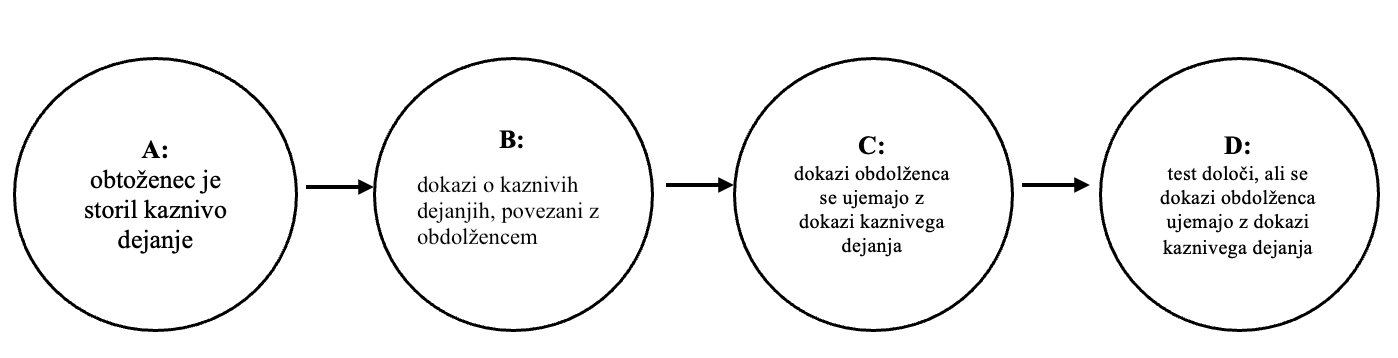
\includegraphics[scale=0.60]{slika_3.png}
   \caption{Vzorčna veriga dokazov}
\end{figure}
\\
Ta analiza je močno odvisna od pojma »pogostost ujemajočih se lastnosti«, označenega kot $F$(lastnosti). Ta se včasih imenuje
tudi »verjetnost naključnega ujemanja«. V našem vzročno-posledičnem okviru je $F$(lastnosti) enakovreden bolj formalno opredeljeni verjetnosti
$P(C \lvert \neg B)$, t.j. verjetnost, da oseba, ki ni vpletena v kaznivo dejanje, po naključju zagotovi dokaze, ki se ujemajo.\\\\
S tem vzročno-posledičnim okvirom lahko opišemo vrsto različnih pogostih zmot, ki so posledica napačnega razumevanja pogojne verjetnosti:\\
\textit{Tožilčeva zmota}: pri tem enačimo $P(C \lvert \neg B)$ s $P(\neg A \lvert C)$. Presega napako predhodne verjetnosti, saj si jo lahko 
predstavljamo kot dopolnitev te napake z dodatno napačno predpostavko $P(A) = P(B)$.\\\\
\textit{Napaka verjetnosti $P(\text{drugo ujemanje})$}: gre za zmoto, ko verjetnost $P(C \lvert \neg B)$ enačimo z verjetnostjo
(imenujmo jo $q$), da ima vsaj en nedolžen član populacije ustreza dokazom. Posledica te napake je običajno močno pretiravanje z vrednostjo
dokaza $C$.\\\\
\textit{Zanemarjanje predhodnih verjetnosti}: to pomeni preprosto neupoštevanje predhodnih vrednosti, kot sta $P(A)$ in $P(B)$. Na splošno
se za zmoto zanemarjanja osnovne stopnje šteje, kadar je verjetnost dogodka podcenjena, ker dogodek ni tako nenavaden, kot se zdi,
ali precenjena, ker je dogodek bolj nenavaden, kot se zdi.\\\\
\textit{Napaka pri številčnem preračunavanju}: pri tem gre za zamenjavo vrednosti $P(C \lvert \neg B)$ s pričakovanim številom drugih oseb,
ki bi jih bilo treba testirati, preden bi našli ujemanje. Ta zmota prav tako pretirava z vrednostjo dokaza $C$.\\\\
\textit{Pričakovane vrednosti, ki pomenijo edinstvenost}: če je velikost populacije približno enaka $1/P(\neg B \lvert C)$, potem mora biti
obdolženec edini primerek. Binomski izrek pokaže, da obstaja več kot 25\% verjetnost, da bosta v populaciji, katere velikost je $1/P(\neg B \lvert C)$,
vsaj dva ujemanja.\\\\
\textit{Zmota obrambnega odvetnika}: to se zgodi, ko se dokaz $C$ šteje za nepomembnega, ker visoka predhodna verjetnost $P(\neg A)$ (kar
se zgodi, če je na primer potencialno število osumljencev zelo veliko) še vedno povzroči visoko verjetnost $P(\neg B \lvert C)$. \\\\
\textit{Napaka baze podatkov obrambnega odvetnika}: za to napako gre, kadar verjetnost $P(\neg B \lvert C)$ temelji na drugačni populaciji,
kot jo določa $P(B)$ ali $P(A)$.\\\\
\textit{Zasliševalčeva zmota}: v tem primeru je dokaz neposredno priznanje krivde. Če to ni potrjeno, to pomeni, da uporabljamo $P(D \lvert A)$ za
informiranje $P(A \lvert D)$. Napaka je, da ne upoštevamo $P(D \lvert \neg A)$. Če je $P(D \lvert A) \leq P(D \lvert \neg A)$, potem dokaz
nima vrednosti.\\\\

%%%%%%%%%%%%%%%%%%%%%%%%%%%%%%%%%%%%%%%%%%%%%%%%%%%%%%%%%%%%%%%%%%%%%%%%%%%%%%%%%%%%%%%%%%%%%%%%%%%%%%%%%%%%%%%%%%%%%%%%%%%%%%%%%%%%%%%%%%%%%%
%%%%%%%%%%%%%%%%%%%%%%%%%%%%%%%%%%%%%%%%%%%%%%%%%%%%%%%%%%%%%%%%%%%%%%%%%%%%%%%%%%%%%%%%%%%%%%%%%%%%%%%%%%%%%%%%%%%%%%%%%%%%%%%%%%%%%%%%%%%%%%
\section{Načini za izogib zmotam}
V zadnjih letih je statistika in verjetnost v kazenskem pravu napredovala. Sodniki, tožilstvo in porota se zavedajo nerazumevanja te znanosti, zato 
je statistika čedalje bolj vpletena že v učne programe pravnih fakultet, kar pripomore k boljšemu razumevanju statističnih analiz. Kljub temu so seveda 
zmote še vedno prisotne. V začetku dela sem omenila, da je razlaga statistične analize odvisna od vprašanj odvetnika, pri čemer veliko za izboljšanje 
ne moremo storiti. Poleg tega morajo biti statistični oziroma forenzični znanstveniki previdni z razlago, kajti ne smejo poseči v poroto. Torej kako 
se dejansko izognimo zmotam in s tem ne posežemo v pravna pravila na sodiščih. 

%%%%%%%%%%%%%%%%%%%%%%%%%%%%%%%%%%%%%%%%%%%%%%%%%%%%%%%%%%%%%%%%%%%%%%%%%%%%%%%%%%%%%%%%%%%%%%%%%%%%%%%%%%%%%%%%%%%%%%%%%%%%%%%%%%%%%%%%%%%%%%
\subsection{Izogib zmotam z uporabo razmerja verjetnosti}

%%%%%%%%%%%%%%%%%%%%%%%%%%%%%%%%%%%%%%%%%%%%%%%%%%%%%%%%%%%%%%%%%%%%%%%%%%%%%%%%%%%%%%%%%%%%%%%%%%%%%%%%%%%%%%%%%%%%%%%%%%%%%%%%%%%%%%%%%%%%%%
\subsection{Izogibanje zmotam z uporabo Bayesovih omrežij}
Ker je največkrat težava v tem, da se večina odvetnikov in sodnikov ob pogledu na verjetnostne izračune in statistično analizo dokazov, ustraši, se mi 
zdijo Bayeosova omrežja dober predlog za predstavitev verjetnostnih izračunov. \\\\
Bayesova omrežja pomagajo določiti ustrezne verjetnostne formule, ne da bi prikazali njihovo polno algebrsko obliko, in omogočajo
skoraj popolno avtomatizacijo potrebnih verjetnostnih izračunov.\\\\
Bayesova omrežja, ki temeljijo na Bayesovi teoriji in teoriji grafov, ponujajo forenzičnim znanstvenikom več prefinjenih možnosti. Tem metodam
se daje poseben poudarek, kadar je treba med konkurenčnimi hipotezami izbrati najverjetnejšo, izbira pa mora biti podprta z znanstveno utemeljeno
argumentacijo. Primerna so za analizo dogodka, ki se je zgodil, in napovedovanje verjetnosti, da je k temu prispeval katerikoli od več možnih
znanih vzrokov. Prednosti Bayesovih mrež se najbolj izrazito pokažejo na zapletenih področjih z več spremenljivkami. Kriminalistične aplikacije
Bayesovih omrežij segajo od prepoznavanja storilcev, posameznih in kompleksnih konfiguracij različnih vrst sledi ter problemov sklepanja, ki
vključujejo rezultate analiz DNK.\\
Ti grafični modeli verjetnosti bistveno izboljšajo vrednotenje verjetnostnih razmerij, ki se uporabljajo za ocenjevanje znanstvenih dokazov.
Omogočajo, da se lotimo kompleksnejših verjetnostnih analiz, kot bi bilo to mogoče s tradicionalnimi pristopi, kar še posebaj pride prav pri primerih z ogromno doazi. \\\\
Struktura Bayesovega omrežja v pravnem kontekstu je dovzetna za napačne predpostavke in napake v procesu ustvarjanja. Izbira vozlišč za dokaze je lahko
pristranska glede na to, kakšna vrsta argumenta je predstavljena. Argumenti obrambe ali tožilstva lahko na primer poudarjajo nasprotne sklepe
in zato vključujejo le podskupino dokazov. Če se za izdelavo ne uporablja dosleden okvir, lahko Bayesovo omrežje, ki jih oblikujejo različne stranke za en
primer, kažejo različne rezultate. Pri oblikovanju Bayesovega omrežja za pravno sklepanje ključnega pomena, da se oblikuje omrežje, ki je razumljivo poroti
in sodniku.\\\\
Prikaz Bayesovega omrežja se mora ujemati z intuitivnim pripisovanjem vzročno-posledičnih povezav med končno hipotezo, kot je »Obtoženec je kriv.«, podhipotezo
»Obtoženec je bil na kraju zločina.« in dokazi primera. Poleg težav, ki se pojavijo med postopkom strukturiranja, je problematično tudi sklepanje
iz omrežja, če se izvaja ob napačnih predpostavkah. Verjetnosti, tudi če temeljijo na strokovni presoji, so lahko pristranske zaradi dejavnikov
motenj v postopku pridobivanja podatkov. Metode za sklepanje morajo zato zagotoviti, da se verjetnosti omrežij ne razlagajo napačno kot dejstva in
da se izpostavi dejavnik negotovosti. Primerjati morajo verjetnosti za nasprotujoče si hipoteze in morajo zagotoviti okvir za pravnike, da iz
mreže sklepajo na argumente.

%%%%%%%%%%%%%%%%%%%%%%%%%%%%%%%%%%%%%%%%%%%%%%%%%%%%%%%%%%%%%%%%%%%%%%%%%%%%%%%%%%%%%%%%%%%%%%%%%%%%%%%%%%%%%%%%%%%%%%%%%%%%%%%%%%%%%%%%%%%%%%
%%%%%%%%%%%%%%%%%%%%%%%%%%%%%%%%%%%%%%%%%%%%%%%%%%%%%%%%%%%%%%%%%%%%%%%%%%%%%%%%%%%%%%%%%%%%%%%%%%%%%%%%%%%%%%%%%%%%%%%%%%%%%%%%%%%%%%%%%%%%%%

\end{document}